\chapter{Analysis}
The purpose of this chapter is to compare the SRS data structure to the kd-tree. We are going to perform a variety of tests on the SRS data structure and the kd-tree in order to determine the run-time properties of both, mainly looking at when the SRS data structure performs better than the kd-tree.


In order to compare these two data structure random data will be generated and given as input to both, such that both operate on the exact same data. This random data is generated by making two lists, $X$ and $Y$ with the integers ${0,1,\cdots,n-1}$ and shuffling them both randomly. The $n$ points given to the data structures as input are found by taking the $i$th entry of both $X$ and $Y$ and generating a point with those coordinates. This ensures that all x-coordinates are unique and all y-coordinates are unique.  When running a specific test, different data sets are generated during the test such that one tests is not only performed on a single data set. When the size of a slice has been determined, the search will be performed different places in the data structure such that not only best-case or worst-case scenarios will occur. Finally the average of all the searches are returned as the result of the test.


\section{Vertical and horizontal slices}

Before introducing the graphs, we are going to look at the theoretical run-time of a search query to the kd-tree and the SRS data structure. A search query to the kd-tree has a run-time of $\mathcal{O}(\sqrt{n}+k)$ and a search query to the SRS data structure has a run-time of $\mathcal{O}(\lg n + k \cdot \lg^\epsilon n)$. When increasing the size of a slice, we expect the run-time of the two search queries to be roughly equal at $k \approx \frac{sqrt{n}}{lg^\epsilon n}$ stemming from $\sqrt{n} + k = \lg n + k \cdot \lg^\epsilon n \Leftrightarrow k = \frac{\sqrt{n} - \lg n}{\lg^\epsilon n - 1}$. The $\mathcal{O}(\lg^\epsilon n)$ describes the amount of jumps needed to perform in order to find the identity of a leaf given the identity of a ball in the ball inheritance structure. Thus, the size of $\mathcal{O}(\lg^\epsilon n)$ on how $B$ is chosen in \todo{ref} and which other meassures have been taken in order to lessen the amount of jumps. \todo{Skriv om at vi har målt dem også, og at de er sat ind på en graf - det er de værste hop vi kigger på? eller er det gennemsnittet? Hvad med grafen der viser $\frac{Skæringspunkt}{\frac{\sqrt{n}}{lg^\epsilon n}}$ - skal det være worst $\lg^\epsilon n$ eller gennemsnittet?}

Recall that the SRS data structure treats the two dimensions very differently. Given a rank space search query $\hat{q} = [\hat{x_1}, \hat{x_2}] \times [\hat{y_1}, \hat{y_2}]$, the search algorithm will find the least common ancestor of $\hat{x_1}$ and $\hat{x_2}$. From there, it will find the path to both $\hat{x_1}$ and $\hat{x_2}$ and all leaves between them will be in the range $[x_1, x_2]$. The search algorithm now has to determine which of these leaves contain a point with y-coordinate in $[y_1, y_2]$. This is done by using the ball inheritance structure from each of the fully contained nodes which were found on the path from the least common ancestor to $\hat{x_1}$ and $\hat{x_2}$.

This means that a horizontal slice and a vertical slice will be treated differently by the SRS data structure. The search query of a horizontal slice includes all x-coordinates of the search space, and thus the least common ancestor of $[\hat{x_1}, \hat{x_2}]$ will be the root of the tree. The path from the least common ancestor to $\hat{x_1}$ will only go left which means each level will give a fully contained node. The path from the least common ancestor to $\hat{x_2}$ will only go right, also yielding a fully contained node per level. The tests are to measure how big a slice can become before the kd-tree performs just as well. This means that a slice will start out being very small, $k=5$. Thus, many of the fully contained nodes will have no ball inheritance work. As the slice grows, eventually each node will have one or more balls to follow. The amount of ball inheritance each node is responsible for varies a lot, and therefore the ball inheritance will become somewhat sporadic. But the nature of the ball distribution asserts that if node has two balls or more balls for ball inheritance, these balls will be right next to each.

On the other hand we have the vertical slice. The vertical slice includes all y-coordinates of the search space, and thus the location least common ancestor of $[\hat{x_1}, \hat{x_2}]$ varies a lot dependent on the search query. But the nodes which are marked as fully contained on the path from the least common ancestor to $\hat{x_1}$ and $\hat{x_2}$ will all only contain leaves with points with y-coordinates in $[y_1, y_2]$ which means we have to do ball inheritance on all the balls belonging to fully contained nodes. Thus, the ball inheritance in vertical slices are much more batched together. Comparing a vertical and horizontal slice of the same size, the vertical slice will have good chances of being faster than the horizontal slice. With a lower LCA, the ball inheritance in the vertical slice will have to jump from a lower level than the ball inheritance in the horizontal and the balls are more batched together in the vertical. 

The first thing to be tested is how big the vertical and horizontal slices can become before the SRS data structure performs worse than the kd-tree. We are going to look at the vertical slices first. Below are some graphs showing the running time of a search query to both the SRS and the kd-tree dependent on the size of the slice. Recall from section \todo{ref} that the parameter $B$ could be set such that we could fix the size of the alphabet (and the jumps) in the ball inheritance tree. The graphs below shows results from a SRS data structure configured with $B=2$. 


\begin{figure}[h]
    \centering
    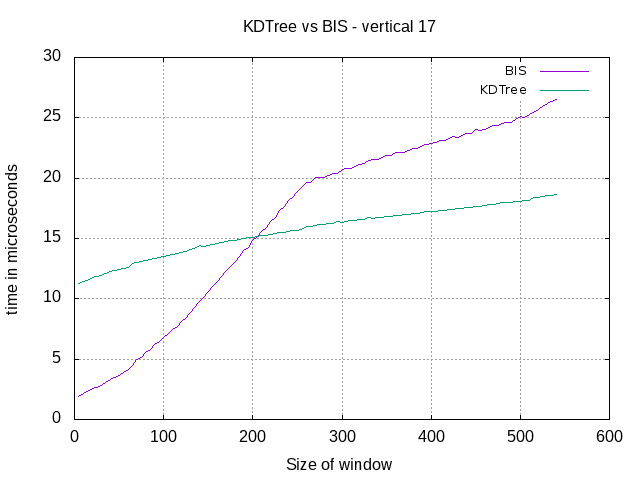
\includegraphics[width = 0.85\textwidth]{pictures/analysis/vert_17.png}
    \caption{vertical slice on SRS and kd-tree - data set size of $n=2^{17}$}\label{fig:vert_17}
\end{figure}

\begin{figure}[h]
    \centering
    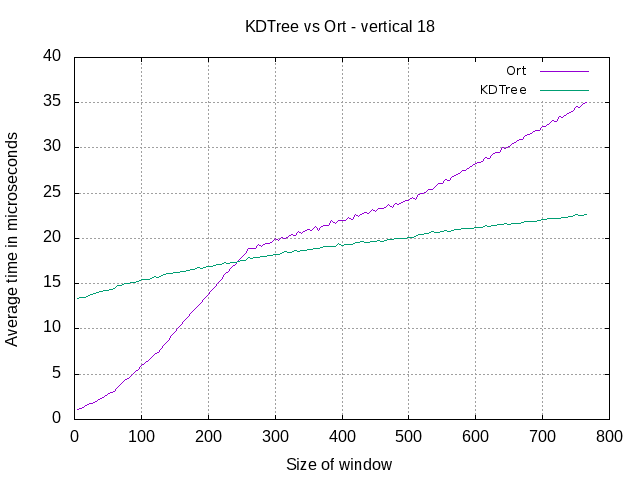
\includegraphics[width = 0.85\textwidth]{pictures/analysis/vert_18.png}
    \caption{vertical slice on SRS and kd-tree - data set size of $n=2^{18}$}\label{fig:vert_18}
\end{figure}

\begin{figure}[h]
    \centering
    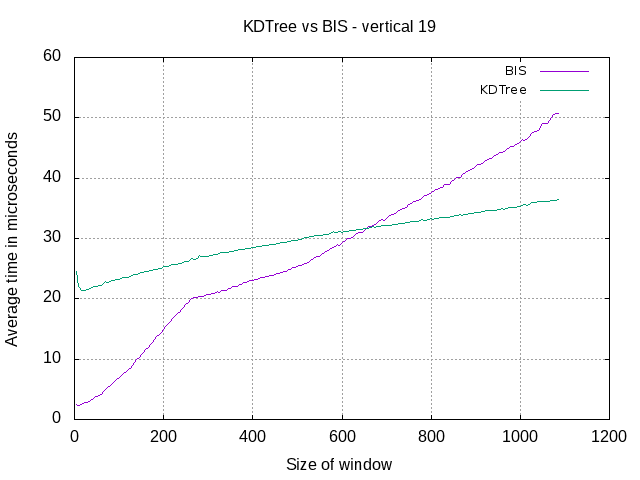
\includegraphics[width = 0.85\textwidth]{pictures/analysis/vert_19.png}
    \caption{vertical slice on SRS and kd-tree - data set size of $n=2^{19}$}\label{fig:vert_19}
\end{figure}

\begin{figure}[h]
    \centering
    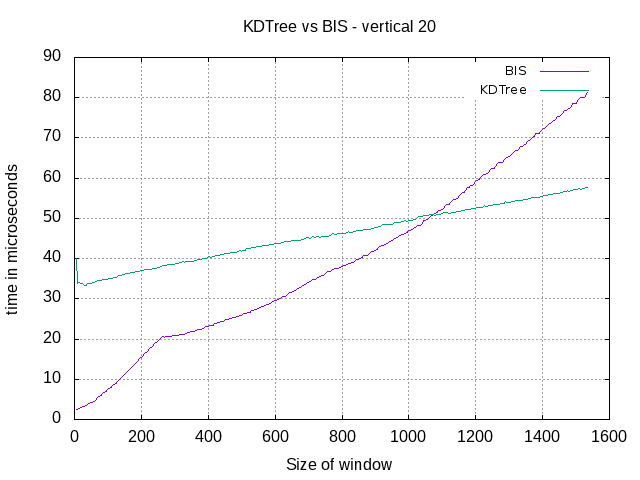
\includegraphics[width = 0.85\textwidth]{pictures/analysis/vert_20.png}
    \caption{vertical slice on SRS and kd-tree - data set size of $n=2^{20}$}\label{fig:vert_20}
\end{figure}

\begin{figure}[h]
    \centering
    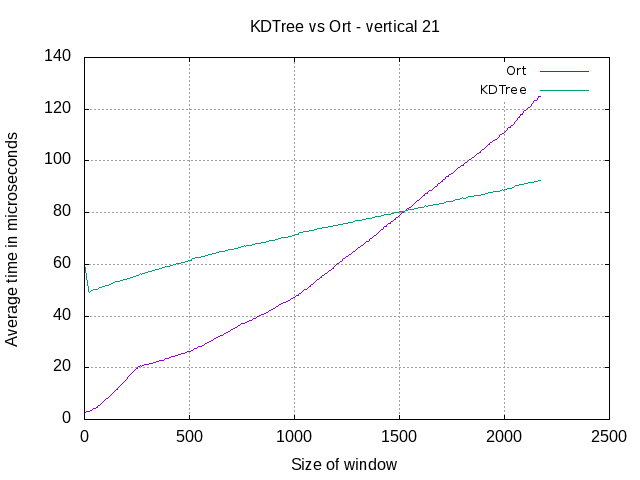
\includegraphics[width = 0.85\textwidth]{pictures/analysis/vert_21.png}
    \caption{vertical slice on SRS and kd-tree - data set size of $n=2^{21}$}\label{fig:vert_21}
\end{figure}

\begin{figure}[h]
    \centering
    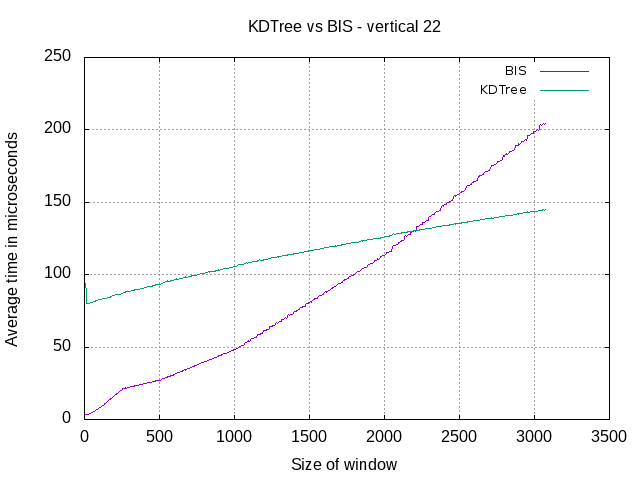
\includegraphics[width = 0.85\textwidth]{pictures/analysis/vert_22.png}
    \caption{vertical slice on SRS and kd-tree - data set size of $n=2^{22}$}\label{fig:vert_22}
\end{figure}

\begin{figure}[h]
    \centering
    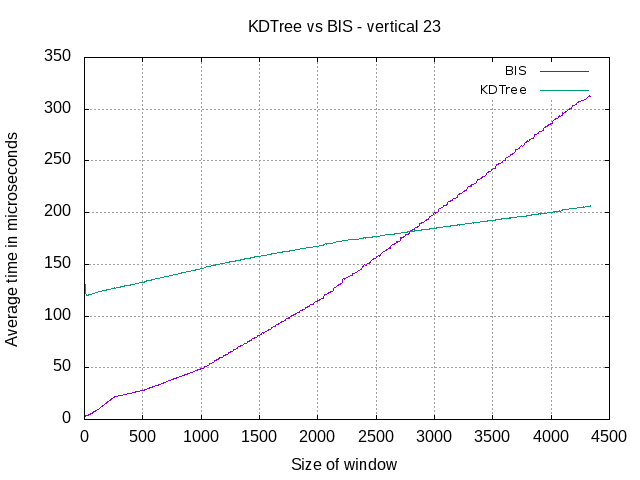
\includegraphics[width = 0.85\textwidth]{pictures/analysis/vert_23.png}
    \caption{vertical slice on SRS and kd-tree - data set size of $n=2^{23}$}\label{fig:vert_23}
\end{figure}

\clearpage

Across these graphs, there is a very noticable change in slope at around $k=256$ for the running time of a search query to the SRS data structure. Since $B=2$, we have a big jump at level $2^3 = 8$ which allows the ball inheritance to jump from level $8$ to a leaf in one jump. This means that the average amount of jumps per result will decrease and thus the running time will not increase as fast as before. At around $k=512$ the running-time resumes its normal behaviour. On average, the ball inheritance structure does not use the big jump at level $8$ directly anymore, resulting in a couple of steps before reaching level $8$. Since the graph shows the average run-time of different configurations of the same slice on different data sets, not all of the searches will hit level $8$ from $k>256$, but the main tedency is to. \todo{forklar tidligere - at vi snakker om main tendency, ikke hvad den er garanteret at gøre}. This tendency is described at figure~\ref{fig:jump_vert_17} and figure~\ref{fig:jump_vert_20}. We see how the graph has a local maximum at around $k=256$ and then the average amount of jumps per result decreases until $k=512$ where it starts increasing at steady level again. Figure~\ref{fig:level_vert_17} and figure~\ref{fig:level_vert_20} describes the highest level of a fully contained node. We see between $k=256$ and $k=512$ that the maximum is level $8$ and the minimum is level $7$ and that the average level increases meaning more and more fully contained node starts using level $8$. Since we $B=2$, there is a $2$-jump every $2$ levels, a $4$-jump every $4$ levels, a $8$-jump every $8$ levels and a $16$-jump every $16$ levels. This means that level $7$ the ball inheritance structure needs $3$ jumps to reach a leaf. This is why such a noticable local maximum exits on figure~\ref{fig:jump_vert_17} and figure~\ref{fig:jump_vert_20}. The jumps per results eases off because from level $8$ there is $1$ jump, from level $9$ there are $2$ jumps and from level $10$ there are $2$ jumps. Levels $11, 13, 14$ have $3$ jumps, and at level $15$ another local maximum is going to be found with $4$ jumps, just before level $16$ with $1$ jump to the leaves. However, $k=2^{16}=65,536$ is not likely to be a place where the SRS data structure performs better than the kd-tree unless we have a enormous data set \todo{regn på det}. \todo{Sæt grafer ind for større $n$}

Looking at figure~\ref{fig:level_vert_17} we see that when we reach $k=256$ the minimum highest level rises to $7$ and the maximum highest level rises to $8$. In order to write the sum of $256<k<512$ we will need to at least level $7$ because we need the two fully included nodes from level $7$ giving us $2*2^7 = 2^8 = 256$ nodes. If the least common ancestor is found at level $9$ the first fully contained node can be found at level $7$. If all the levels from level $7$ to level $1$ only have fully contained nodes, we get $k = 2*2^1 + 2*2^2 + \cdots + 2*2^7 = 508$. This is not enough to write $512$, and thus somewhere between $k=256$ and $k=512$, the search algorithm will begin using level $10$ as the least common ancestor. This is also very dependent on how the slice covers the subtrees of the least common ancestor. If the slice hits the least common ancestor right in the middle, such that the left subtree and the right subtree of the least common ancestor is of the exact same size, the level of the highest fully included node will be lower. If the slice hits the least common ancestor such there is an imbalance in the size between the left subtree and right subtree of the least common ancestor, the level of the highest fully included node will be higher, because now one subtree has to account for a bigger portion of the slice and will have to use bigger pieces. And when a subtree contains $2^8 = 256$ leaves it will have access to the jump at level $8$. The maximum level of figure~\ref{fig:level_vert_17} is explained by the fact that it is not possible to write the sum of $k<512$ using $512$ as a summand. Recall that a vertical slice conceptually only searches for the x-coordinates of the points. All the y-coordinates are already known to be included, Thus, when a node is fully included, we get all of points in its subtree.   \todo{Omformuler og sæt sammen med afsnittet fra før lige ovenover da du skriver nogenlunde det samme - bare i to forskellige tankegange}\todo{Lav en lignede figur som figur 3.2 til at forklare konceptet}


\begin{figure}[h]
    \centering
    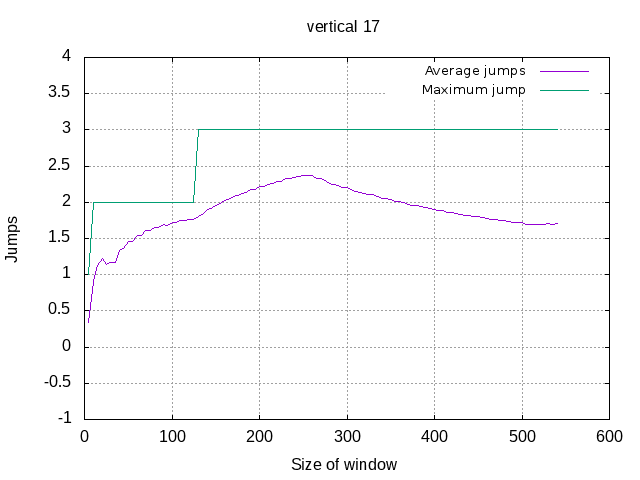
\includegraphics[width = 0.85\textwidth]{pictures/analysis/jump_vert_17.png}
    \caption{Size of jumps - data set size of $n=2^{17}$. 'Average jumps' is the average of all the jumps performed normalized by the size of the slice}\label{fig:jump_vert_17}
\end{figure}

\begin{figure}[h]
    \centering
    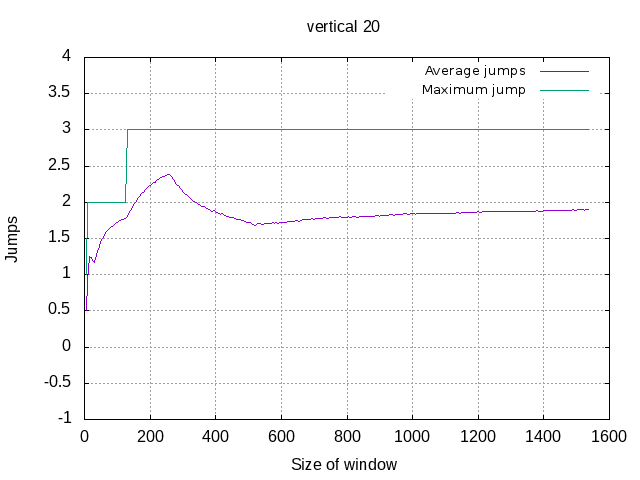
\includegraphics[width = 0.85\textwidth]{pictures/analysis/jump_vert_20.png}
    \caption{Size of jumps - data set size of $n=2^{20}$. 'Average jumps' is the average of all the jumps performed normalized by the size of the slice}\label{fig:jump_vert_20}
\end{figure}



\begin{figure}[h]
    \centering
    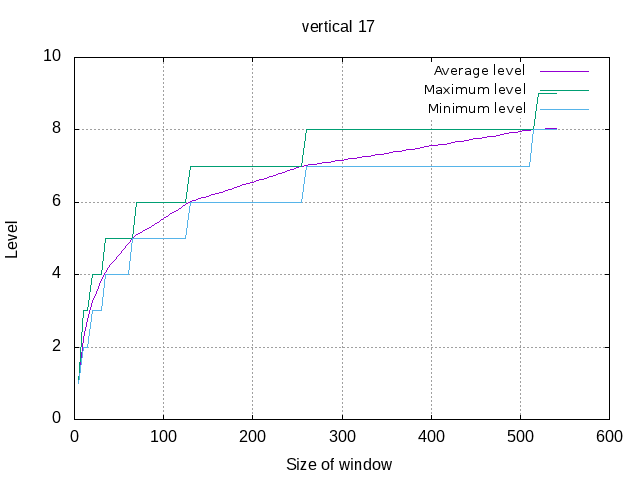
\includegraphics[width = 0.85\textwidth]{pictures/analysis/level_vert_17.png}
    \caption{Level of first fully contained node - data set size of $n=2^{17}$.}\label{fig:level_vert_17}
\end{figure}

\begin{figure}[h]
    \centering
    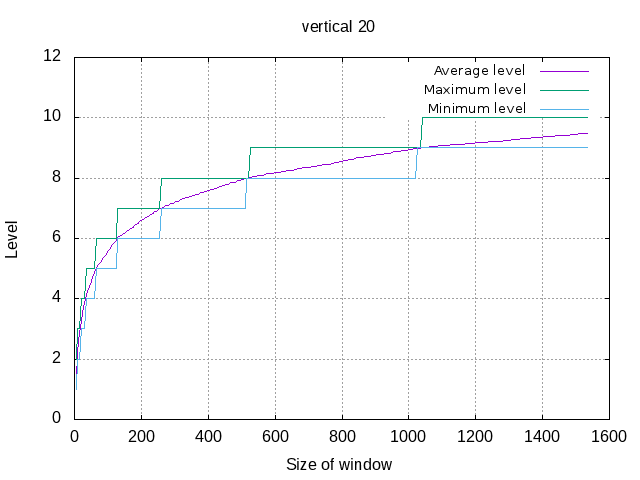
\includegraphics[width = 0.85\textwidth]{pictures/analysis/level_vert_20.png}
    \caption{Level of first fully contained node - data set size of $n=2^{20}$.}\label{fig:level_vert_20}
\end{figure}


To summarize the graphs for vertical slices, figure~\ref{fig:vert_intersection} shows the size of the slice at the point of intersection between the running-time of a search to the SRS and the kd-tree for each $n$ tested. Recall the theory described above where it was described how the intersection point should theoretically be $k_{theoretical} = \frac{\sqrt{n} - \lg n}{\lg^\epsilon n - 1}$. Figure~\ref{fig:vert_theory} and figure~\ref{fig:vert_theory_worst_jump} show $\frac{k_{actual}}{k_{theoretical}}$. One graph uses $\lg^\epsilon n$ as the average jump per result while the other uses $\lg^\epsilon n$ as the worst case jump. If the graph is below $1$ it means that the SRS data structure performed worse than theoretically expected and if it above $1$ it means that the SRS data structure performed better than theoretically expected. The increase in the slope of the graph on figure~\ref{fig:vert_intersection} can be described by the decrease in the average jumps per results as seen on figure~\ref{fig:vert_jumps_per_lgn}. This big drop in figure~\ref{fig:vert_jumps_per_lgn} can be explained by looking at figure~\ref{fig:vert_18} and figure~\ref{fig:vert_19}. The intersection between the running time of the SRS and the kd-tree on figure~\ref{fig:vert_18} is just prior to the running time of the SRS changing its slope drastically. At figure~\ref{fig:vert_19} we see the of the running time of the SRS has changed prior to its intersection with the running time of the kd-tree. With access to the jump from level $8$, the average amount of jumps per result has been lowered. This can also be noted from figure~\ref{fig:vert_intersection} seeing that at $\lg n = 18$ the point of intersection is around $k=250$.

\begin{figure}[h]
    \centering
    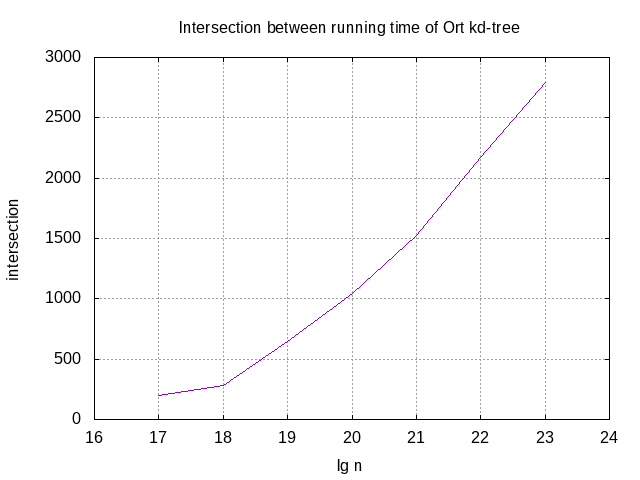
\includegraphics[width = 0.85\textwidth]{pictures/analysis/vert.png}
    \caption{Vertical slices, intersection between running time of SRS and kd-tree}\label{fig:vert_intersection}
\end{figure}


\begin{figure}[h]
    \centering
    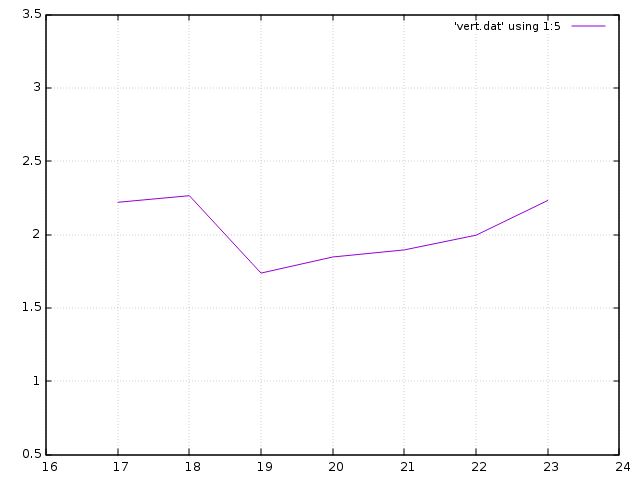
\includegraphics[width = 0.85\textwidth]{pictures/analysis/vert_jumps_per_lgn.png}
    \caption{Vertical slices, average jumps per result at the point of intersection between the running time of the SRS and the kd-tree}\label{fig:vert_jumps_per_lgn}
\end{figure}


\begin{figure}[h]
    \centering
    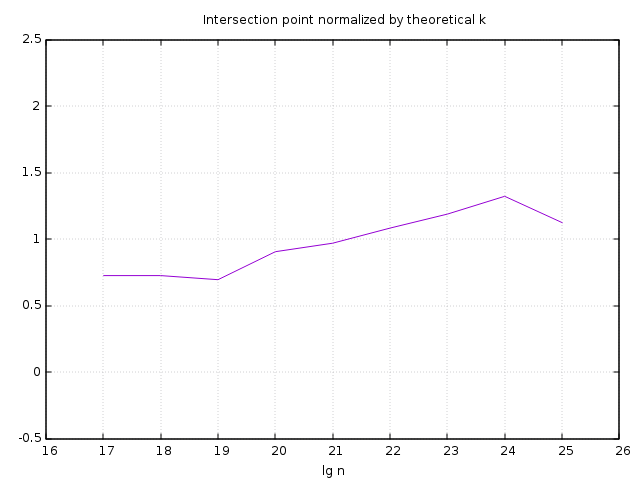
\includegraphics[width = 0.85\textwidth]{pictures/analysis/vert_theory.png}
    \caption{Vertical slices, intersection between running time of SRS and kd-tree normalized by $k_{theoretical}$ with $\lg^\epsilon n$ being the average amount of jumps per result}\label{fig:vert_theory}
\end{figure}


\begin{figure}[h]
    \centering
    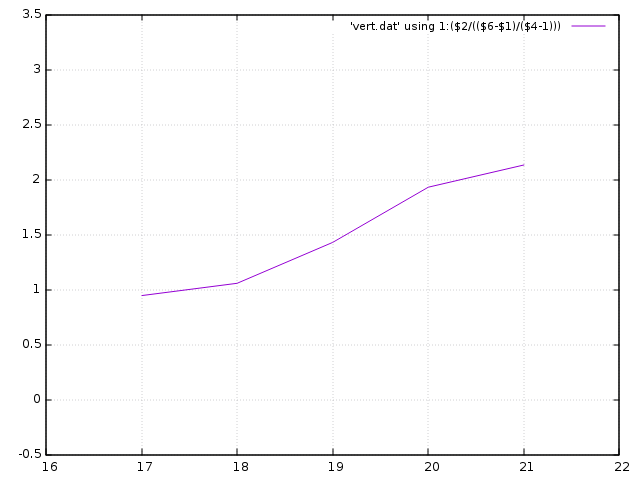
\includegraphics[width = 0.85\textwidth]{pictures/analysis/vert_theory_worst_jump.png}
    \caption{Vertical slices, intersection between running time of SRS and kd-tree normalized by $k_{theoretical}$ with $\lg^\epsilon n$ being the worst amount of jumps per result}\label{fig:vert_theory_worst_jump}
\end{figure}


We are now going to look at the graphs for the horizontal slices. Recall that when a search query is a horizontal slice, the least common ancestor will be the root of the tree. In $[\hat{x_1}, \hat{x_2}]$, $\hat{x-1}$ will be the leftmost leaf and $\hat{x_2}$ will be the rightmost leaf. From the root to $\hat{x_1}$ and $\hat{x_2}$ there will many fully included nodes, $2$ per level to be exact, which means there will be many different nodes performing small amount of balls inheritance look-ups. Since the points are ordered by their y-coordinate in the root before distribution, and the fact that they keep this order while being distributed means that when increasing the range from $[y_1, y_2]$ to $[y_1, y_2 + 5]$ it is more likely that these $5$ new points will be found from a higher level where the range $[y_1, y_2]$ already had jumps from. It is much likely that a point is stored in a leaf which belongs to a fully included node from level $8$ with $256$ leaves than belonging to a node from level $2$ with $4$ leaves. But since the points are distributed to leaves according to their x-coordinates, it is hard to know the distribution of y-coordinates. When a search query is a horizontal slice, the position of $\hat{y_1}$ and $\hat{y_2}$ will be found on the bit vector of the root node. These position will be updated using the succint rank query while traveling from the root node to the leftmost leaf and the rightmost leaf in the tree.

\begin{figure}[h]
    \centering
    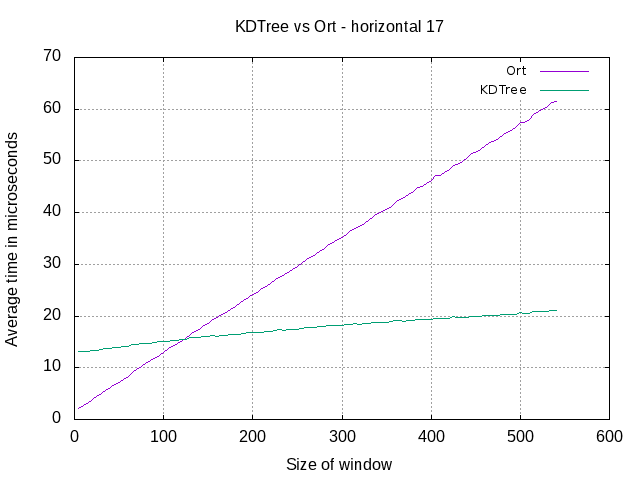
\includegraphics[width = 0.85\textwidth]{pictures/analysis/hori_17.png}
    \caption{Horizontal slice on SRS and kd-tree - data set size of $n=2^{17}$}\label{fig:hori_17}
\end{figure}

\begin{figure}[h]
    \centering
    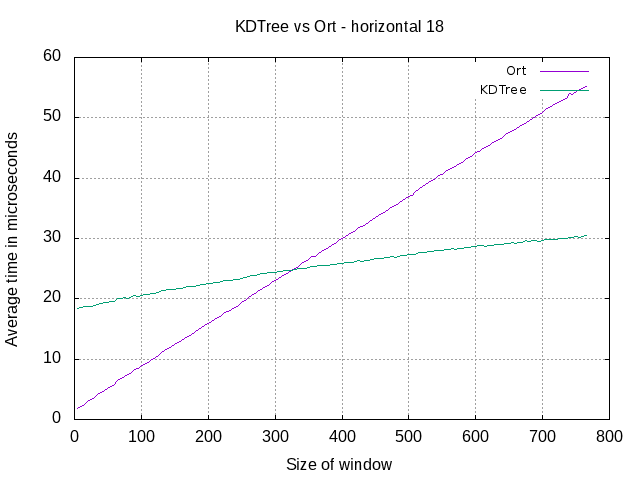
\includegraphics[width = 0.85\textwidth]{pictures/analysis/hori_18.png}
    \caption{Horizontal slice on SRS and kd-tree - data set size of $n=2^{18}$}\label{fig:hori_18}
\end{figure}

\begin{figure}[h]
    \centering
    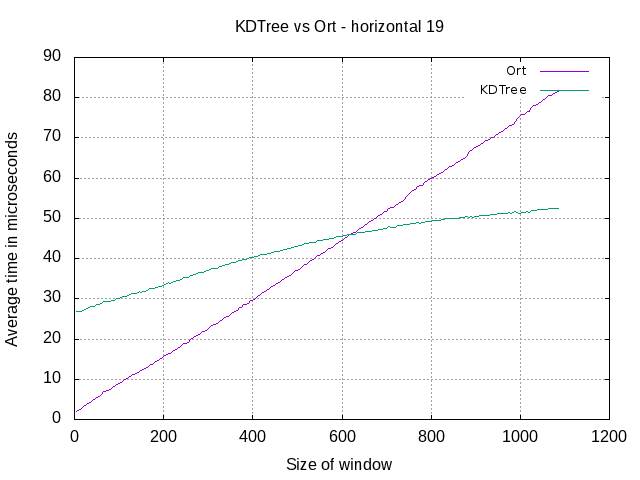
\includegraphics[width = 0.85\textwidth]{pictures/analysis/hori_19.png}
    \caption{Horizontal slice on SRS and kd-tree - data set size of $n=2^{19}$}\label{fig:hori_19}
\end{figure}

\begin{figure}[h]
    \centering
    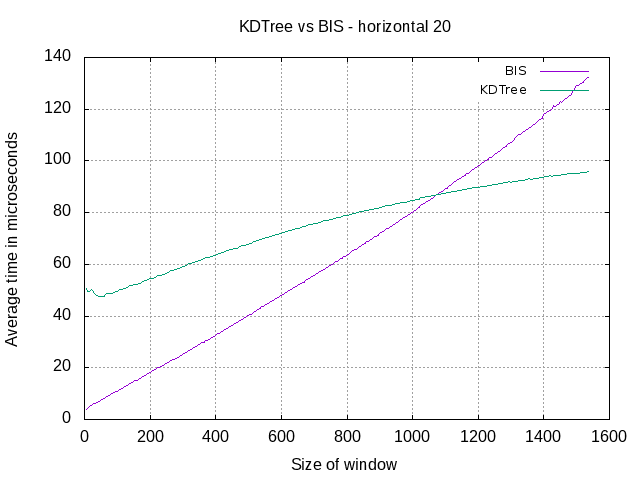
\includegraphics[width = 0.85\textwidth]{pictures/analysis/hori_20.png}
    \caption{Horizontal slice on SRS and kd-tree - data set size of $n=2^{20}$}\label{fig:hori_20}
\end{figure}

\begin{figure}[h]
    \centering
    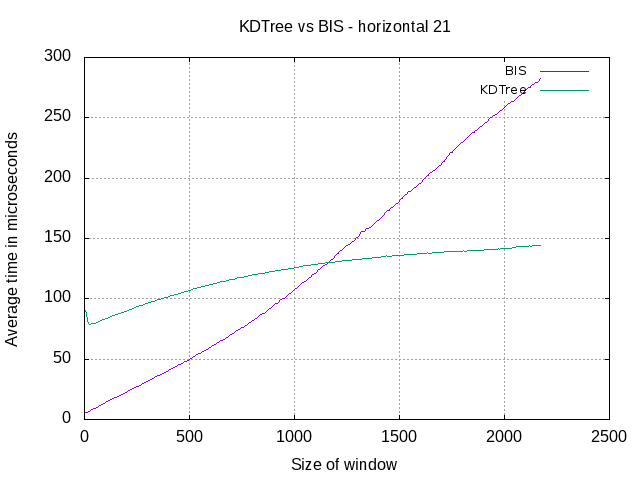
\includegraphics[width = 0.85\textwidth]{pictures/analysis/hori_21.png}
    \caption{Horizontal slice on SRS and kd-tree - data set size of $n=2^{21}$}\label{fig:hori_21}
\end{figure}

\begin{figure}[h]
    \centering
    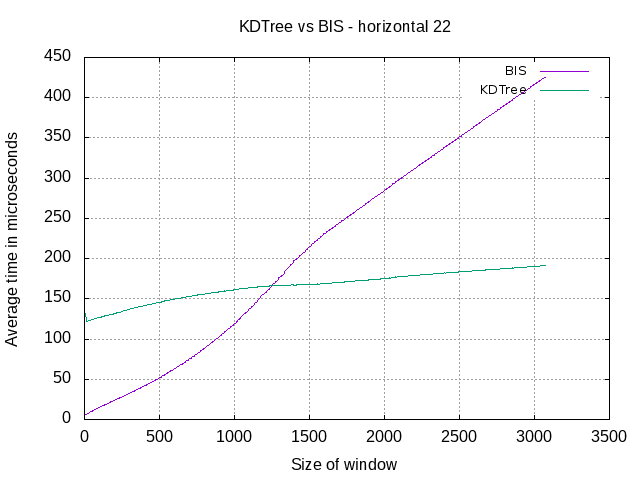
\includegraphics[width = 0.85\textwidth]{pictures/analysis/hori_22.png}
    \caption{Horizontal slice on SRS and kd-tree - data set size of $n=2^{22}$}\label{fig:hori_22}
\end{figure}

\begin{figure}[h]
    \centering
    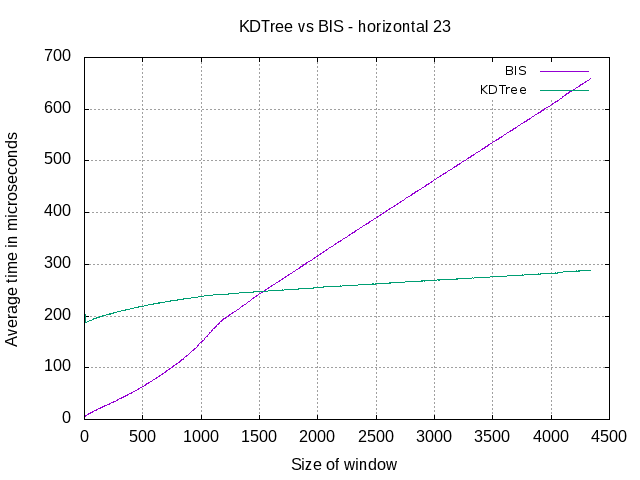
\includegraphics[width = 0.85\textwidth]{pictures/analysis/hori_23.png}
    \caption{Horizontal slice on SRS and kd-tree - data set size of $n=2^{23}$}\label{fig:hori_23}
\end{figure}

\todo{Hvorfor knækker grafen mellem $512$ og $1024$? Hvorfor er kd-træet mærkeligt dårligt inden $k=10$? HORI}

To summarize these graphs for horizontal slices, figure~\ref{fig:hori_intersection} shows the size of the slice at the point of intersection between the running-time of a search to the SRS and kd-tree for each $n$ tested.

\begin{figure}[h]
    \centering
    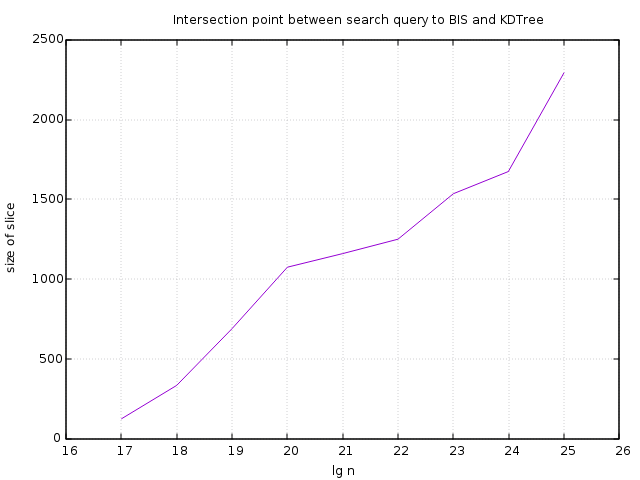
\includegraphics[width = 0.85\textwidth]{pictures/analysis/hori.png}
    \caption{Horizontal slices, intersection between running time of SRS and kd-tree}\label{fig:hori_intersection}
\end{figure}


\begin{figure}[h]
    \centering
    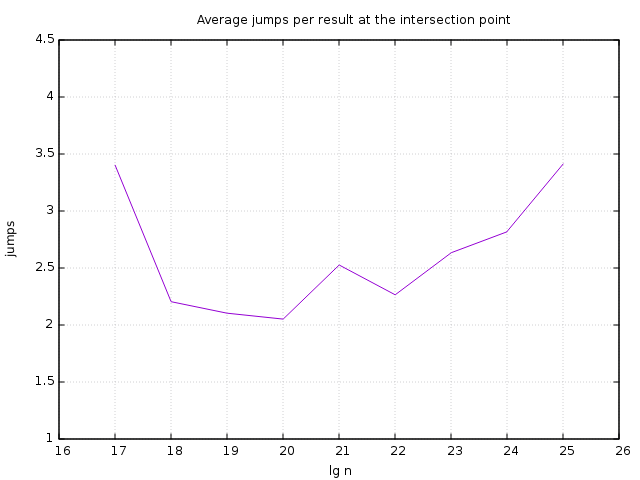
\includegraphics[width = 0.85\textwidth]{pictures/analysis/hori_jumps_per_lgn.png}
    \caption{Horizontal slices, average jumps per result at the point of intersection between the running time of the SRS and the kd-tree}\label{fig:hori_jumps_per_lgn}
\end{figure}


\begin{figure}[h]
    \centering
    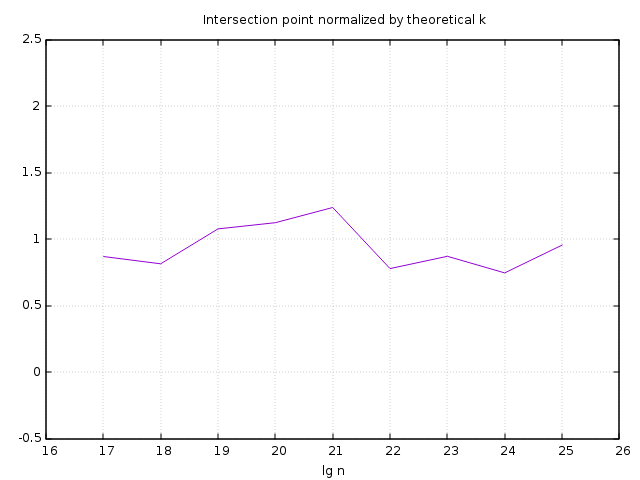
\includegraphics[width = 0.85\textwidth]{pictures/analysis/hori_theory.png}
    \caption{Horizontal slices, intersection between running time of SRS and kd-tree normalized by $k_{theoretical}$ with $\lg^\epsilon n$ being the average amount of jumps per result}\label{fig:vert_theory}
\end{figure}


\begin{figure}[h]
    \centering
    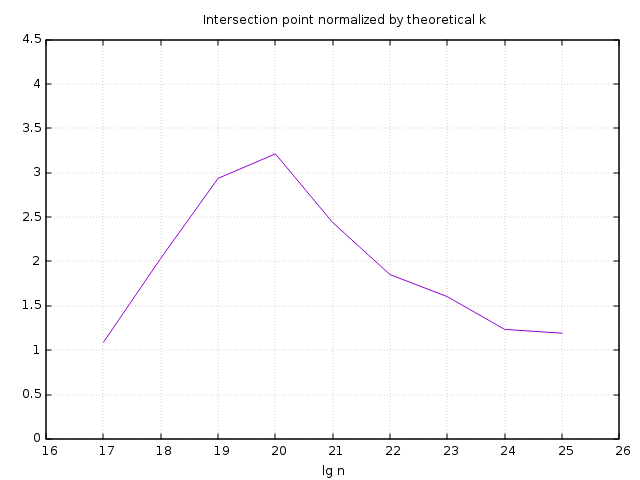
\includegraphics[width = 0.85\textwidth]{pictures/analysis/hori_theory_worst_jump.png}
    \caption{Horizontal slices, intersection between running time of SRS and kd-tree normalized by $k_{theoretical}$ with $\lg^\epsilon n$ being the average amount of jumps per result}\label{fig:vert_theory}
\end{figure}

\section{Comparision of SRS and kd-tree with a constantly small $k$}

Grafer kommer
